\usecasebase{Visualizzazione della notifica di richiesta di inserimento \textit{feedback}}
\label{usecase:Visualizzazione della notifica di richiesta di inserimento feedback}

\begin{figure}[h]
	\centering
	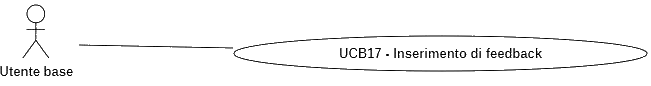
\includegraphics[width=0.9\textwidth]{./uml/UCB17.png} 
	\caption{Visualizzazione della notifica di richiesta di inserimento \textit{feedback}}
	\label{fig:UCB17}
  \end{figure}

\begin{itemize}
	\item \textbf{Attore principale:} Utente base.


	\item \textbf{Precondizione:} L'Utente ristoratore ha cambiato lo stato della prenotazione in "Terminata"(vedi \autoref{usecase:Termina prenotazione}).


	\item \textbf{Postcondizione:} L'Utente base visualizza la notifica in cui
	      gli viene richiesto se vuole lasciare un \textit{feedback} ad una prenotazione.

	\item \textbf{Scenario principale:}
	      \begin{enumerate}
		      \item Il Sistema rivela un cambiamento dello stato della prenotazione;
		      \item Il Sistema invia all'Utente base relativo a questa prenotazione una notifica in cui lo invita a lasciare un \textit{feedback};
		      \item L'Utente base visualizza la notifica e dunque può lasciare un \textit{feedback} (vedi \autoref{usecase:Inserimento di feedback e recensioni}).
	      \end{enumerate}
\end{itemize}
